% Chapter 2

\chapter{Scope} % Main chapter title
\label{Chapter2} % For referencing the chapter elsewhere, use \ref{Chapter2} 

%This chapter presents the scope of the thesis. The main work of this research 
%is to study the offline analysis of ScaRR's model.
%\ft{``Section~\ref{sec:implementation}'' is always capital letter, and add
%a tilde ``\textasciitilde'' in between.}
%In Section~\ref{sec:implementation}, we presents the scope of implementation. 
%Section
%\ref{sec:analysis} discusses the scope of the analysis.

%\section{Implementation}
%\label{sec:implementation}

%\begin{figure}[t]
%\centerline{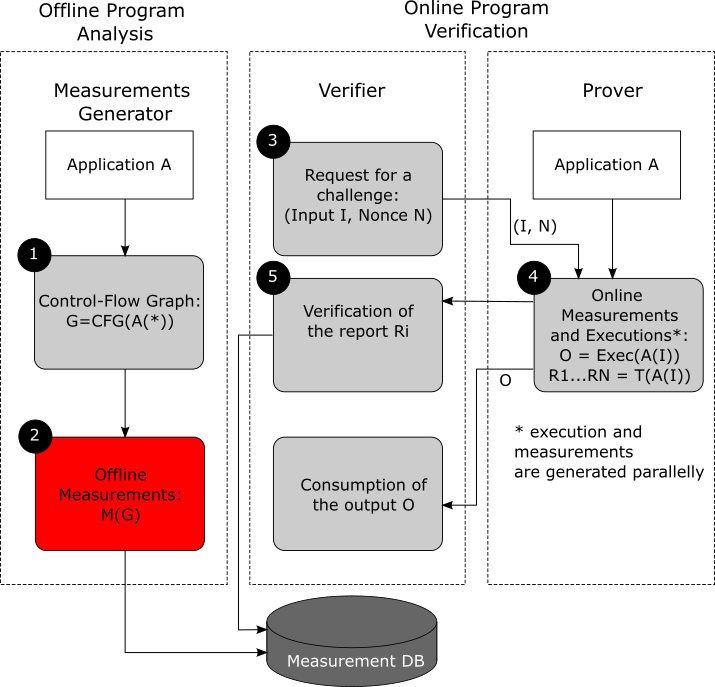
\includegraphics[scale=.5]{Figures/02/scarr-system-overview.png}}
%\caption{ScaRR System Overview}
%\label{fig:scarr-system-overview}
%\end{figure}

\ft{ALWAYS PRESENT!!! CHECK ALL THE TEXT}

%In Chapter \ref{Chapter1}, we presented different runtime remote attestation
%approaches. In learning the different models of runtime remote attestation, we
%implemented one of the model: 
The main work of this research is to study the offline analysis of ScaRR's 
model~\cite{toffaliniScaRRScalableRuntime2019} over a set of programs written 
in C \textbackslash C++. 
Specifically, we write a tool to extract offline measurement using the ScaRR 
control-flow model, verify the scalability of the algorithm, and study its 
limitation.

To sum up, the main contributions of this thesis are:
\begin{enumerate}
	\item propose an implementation of ScaRR's offline measurement extractor.
	\item verify the scalability of ScaRR's offline measurement algorithm.
	\item study the algorithm limitation.
\end{enumerate}

\section{Outline}
\label{sec:outline}

\ft{here, make a list about the content of the following chapter as a list. For 
instance:}

\vspace{0.5cm}
\noindent \textbf{Chapter~\ref{Chapter3}:} We discuss the background.

\vspace{0.5cm}
\noindent \textbf{Chapter~\ref{Chapter4}:} \dots